\documentclass[xcolor=dvipsnames, 11pt]{beamer}

\usetheme{Warsaw}
\useoutertheme{split}
\setbeamertemplate{headline}{}

\usepackage{ucs}
\usepackage[utf8x]{inputenc}
\usepackage[greek,english]{babel}
\usepackage{hyperref}
\usepackage{tcolorbox}
\usepackage{alphabeta}
\usepackage{amsmath}
\usepackage{amsthm}
\usepackage{caption}
\usepackage{algorithm2e}
\tcbuselibrary{theorems}

\newtcbtheorem{mydefinition}{\el Ορισμός}%
{colback=blue!5,colframe=black!15!black,fonttitle=\bfseries}{th}

\newtcbtheorem{mytheorem}{\el Θεώρημα}%
{colback=blue!5,colframe=black!15!black,fonttitle=\bfseries}{th}

\newtcbtheorem[number within=section]{mylemma}{Λήμμα}%
{colback=blue!5,colframe=black!15!black,fonttitle=\bfseries}{th}

\newcommand{\en}{\selectlanguage{english}}
\newcommand{\el}{\selectlanguage{greek}}
\newcommand{\R}{\mathbb{R}}

\setbeamertemplate{itemize items}[ball]
\setbeamertemplate{itemize subitem}[ball]

\begin{document}

\title{Travelling Salesman Problem}
\subtitle{TSP}

\author[\el Σιώρος Βασίλειος, Ανδρινοπούλου Χριστίνα]{\el Σιώρος Βασίλειος \and \el Ανδρινοπούλου Χριστίνα}
\date{\el Απρίλιος, 2020}

\frame{\titlepage}

\begin{frame}
	\frametitle{\el Δομή Παρουσίασης}
	\tableofcontents
\end{frame}

\section{Εισαγωγή}
\begin{frame}
	\frametitle{\el Εισαγωγή}
	\tableofcontents[currentsection]
\end{frame}
\subsection{Ορισμός}
\begin{frame}
	\frametitle{\el Ορισμός}
	\begin{itemize}
		\item \el Κλασσικό πρόβλημα της θεωρητικής επιστήμης των  υπολογιστών. 
		\item \el Ο πωλητής οφείλει να επισκευτεί \en n \el το πλήθος πόλεις για να πουλήσει το εμπόρευμά του.  
		\item \el Ο πωλητής πρέπει να επισκεφτεί την κάθε πόλη ακριβώς μία φορά ακολουθώντας το συντομότερο δρομολόγιο και να επιστρέψει στην πόλη εκκίνισης.
	\end{itemize}
	\begin{figure}
		
\includegraphics[scale=0.3]{images/tsp.png}
		\caption{\en Travelling Salesman Problem - TSP}
	\end{figure}
\end{frame}

\subsection{Εφαρμογές}
\begin{frame}
	\frametitle{\el Εφαρμογές}
	\begin{itemize}
		\item \el Μεταφορές και \en Logistics:
		\begin{itemize}
			\item \el Καθορισμός δρομολογίων σχολικών λεωφορείων
			\item \el Παράδοση τροφίμων σε άτομα που δεν μπορούν να μετακινηθούν από το σπίτι
			\item \el Δρομολόγηση φορτηγών για παραλαβή δεμάτων
			\item \el Εφοδιασμός σε ορόφους καταστημάτων ή σε αποθήκες
		\end{itemize}
		\item \el Βιολογία:
		\begin{itemize}
			\item \en DNA sequencing: οι "πόλεις" είναι DNA strings και η απόσταση είναι τα αποτελέσματα μέτρων σημασιολογικής ομοιότητας
		\end{itemize}
		\item \el Διάστημα:
		\begin{itemize}
			\item \el Ελαχιστοποίηση των καυσίμων που απαιτούνται για την παρατήρηση ουράνιων αντικειμένων
		\end{itemize}	
	\end{itemize}
\end{frame}

\section{Θεωρητική Προσέγγιση}
\subsection{Πολυπλοκότητα}
\begin{frame}
	\frametitle{\el Θεωρητική Προσέγγιση}
	\tableofcontents[currentsubsection]
\end{frame}

\begin{frame}
	\frametitle{\el Πολυπλοκότητα}
	\begin{itemize}
		\item \el Κλάση \(P\)
		\begin{itemize}
			\item \el Προβλήματα για τα οποία έχει βρεθεί αλγόριθμος που για μέγεθος εισόδου \(n\) έχει χρόνο εκτέλεσης χειρότερης περίπτωσης \(Ο(n^k)\), όπου \(k\) κάποια σταθερά είναι. 
		\end{itemize}
		\item \el Κλάση \(NP\)
		\begin{itemize}
			\item \el Προβλήματα για τα οποία δεν έχει ακόμα ανακαλυφθεί αλγόριθμος που να τα επιλύει σε πολυωνυμικό χρόνο.
			\item \el Αλγόριθμοι οι οποίοι αν γνωρίζουν μία πιθανή λύση των προβλημάτων αυτών μπορούν να την επαληθεύσουν σε πολυωνυμικό χρόνο.
		\end{itemize}
	\end{itemize}
\end{frame}

\begin{frame}
	\frametitle{\el Πολυπλοκότητα}
	\begin{itemize}
		\item \el Πολλές φορές τα προβλήματα που ανήκουν στην κλάση \en NP \el μοιάζουν εντυπωσιακά πολύ με κάποιο πρόβλημα που ανήκει στην κλάση \en P.
		\item \el Δεδομένου ενός γράφου \(G = (V,E)\), η εύρεση κύκλου \en Euler \el έχει πολυπλοκότητα \(Ο(|Ε|)\). 
		\item \el H εύρεση κύκλου \en Hamilton, \el είναι \en NP- \el πλήρες πρόβλημα.
	\end{itemize}
\end{frame}

\begin{frame}
	\frametitle{\el Πολυπλοκότητα}
	\begin{itemize}
		\item \(P \subseteq NP\)
		\begin{itemize}
			\item \el Αν ένα πρόβλημα ανήκει στην κλάση \(P\), τότε θα ανήκει και στην κλάση \(NP\)
			\item \el Ένα πρόβλημα που ανήκει στην \(P\) μπορεί να επαληθευτεί σε πολυωνυμικό χρόνο με δεδομένη κάποια λύση.
		\end{itemize} 
		\item \(NP \subseteq P\)
		\begin{itemize}
			\item \el Ούτε έχει επιβεβαιωθεί, όυτε έχει καταρριφθεί.
		\end{itemize}
	\end{itemize}
\end{frame}

\begin{frame}
	\frametitle{\el Πολυπλοκότητα}
	\begin{figure}
		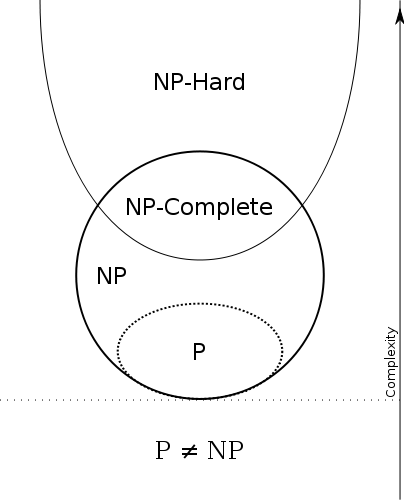
\includegraphics[scale=0.3]{images/complexity_classes.png}
		\caption{\en P \el κλάση και \en NP \el κλάση \\ πηγή: \en https://jcaip.github.io/Reduction-and-Intractibility/}
	\end{figure}
\end{frame}

\begin{frame}
	\frametitle{\el Πολυπλοκότητα}
	\begin{mylemma}{TSP}{}
		Tο πρόβλημα του περιοδεύοντος πωλητή ανήκει στην κλάση NP.	
	\end{mylemma}
	\begin{mylemma}{TSP}{}
		Tο πρόβλημα του περιοδεύοντος πωλητή είναι NP-complete.	
	\end{mylemma}
	\begin{itemize}
		\item \el Δεν περιμένουμε αλγόριθμο που να επιλύει το πρόβλημα σε πολυωνυμικό χρόνο , αλλά κάποιον προσεγγιστικό αλγόριθμο.
	\end{itemize}
\end{frame}

\begin{frame}
	\frametitle{\el Πολυπλοκότητα}
	\begin{itemize}
		\item \el Προσεγγιστικός Αλγόριθμος
		\begin{itemize}
			\item \el Υπολογίζει σχεδόν βέλτιστες λύσεις.
			\item \el Επιτυγχάνει λόγο προσέγγισης \(ρ(n)\), \(n\) το μέγεθος της εισόδου του αλγορίθμου.
			\item \el
			\begin{align*}
				\max\left(\frac{C}{C_{OPT}}, \frac{C_{OPT}}{C}\right) \leq ρ(n)
			\end{align*}  
			όπου \(C\) και \(C_{OPT}\) το κόστος της λύσης του προσεγγιστικού αλγορίθμου και της βέλτιστης λύσης αντίστοιχα.
			\item \el Καλείται \(ρ(n)\)-προσεγγιστικός.			
		\end{itemize}
	\end{itemize}
\end{frame}

\subsection{Μαθηματικό Υπόβαθρο}
\begin{frame}
	\frametitle{\el Θεωρητική Προσέγγιση}
	\tableofcontents[currentsubsection]
\end{frame}

\begin{frame}
	\frametitle{\el Μαθηματικό Υπόβαθρο}
	
\end{frame}

\subsubsection{Γραφήματα}
\begin{frame}
	\frametitle{\el Θεωρητική Προσέγγιση}
	\tableofcontents[currentsubsection]
\end{frame}
\begin{frame}
	\frametitle{\el Γραφήματα}
	\begin{itemize}
		\item \el Βασικά συστατικά ενός γραφήματος είναι:
		\begin{itemize}
			\item \el Κορυφές \(V\)
			\item \el Ακμές \(E\)
		\end{itemize}
		\item \el Οι κορυφές ενώνονται με τη βοήθεια των ακμών και δημιουργούν ένα γράφημα. \\
	\end{itemize}
\end{frame}

\begin{frame}
	\frametitle{\el Γραφήματα}
	\begin{itemize}	
		\item \el Κατευθυνόμενα γραφήματα
		\begin{itemize}
			\item \el Γεωμετρική αναπαράσταση: ένα σύνολο από \(V\) σημεία ενώνονται με \(E\) βέλη.
			\item \el Το \(E\) είναι μία διμελής σχέση.
		\end{itemize}
			
		\item \el Μη κατευθυνόμενα γραφήματα
		\begin{itemize}
			\item \el Γεωμετρική αναπαράσταση: ένα σύνολο από \(V\) σημεία ενώνονται με \(E\) ακμές, που δεν υποδεικνύουν κατεύθυνση. 
			\item \el Το \(E\) είναι σύνολο πολυσυνόλων δύο στοιχείων.
		\end{itemize}		
	\end{itemize}
	\begin{columns}[t]
		\column{.3\textwidth}
		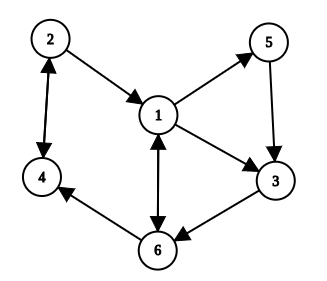
\includegraphics[width=\columnwidth,height=2.5cm]{images/directed_graph_example.png}
		\captionof{figure}{Παράδειγμα κατευθυνόμενου γράφου}
		\column{.3\textwidth}
		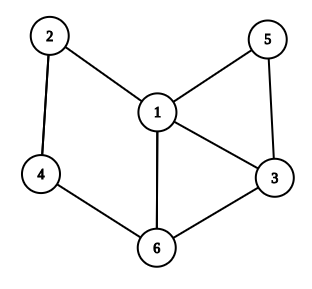
\includegraphics[width=\columnwidth,height=2.5cm]{images/undirected_graph_example.png}
		\captionof{figure}{Παράδειγμα μη κατευθυνόμενου γράφου}
	\end{columns}
\end{frame}

\begin{frame}
	\frametitle{\el Γραφήματα - Μονοπάτια}	
	\begin{itemize}
		\item \el Κατευθυνόμενα Γραφήματα
			\begin{itemize}
				\item \el Μία ακολουθία ακμών \((e_1, e_2,...,e_k)\) όπου η τερματική κορυφή μίας ακμής \(e_j\) ταυτίζεται με την αρχική κορυφή της \(e_{(j+1)}\) καλείται μονοπάτι.
				\item \el Κύκλωμα καλείται το μονοπάτι \((e_1, e_2,...,e_k)\), όπου η τερματική κορυφή της \(e_k\) ακμής συμπίπτει με την αρχική κορυφή της \(e_1\) ακμής. \\
			\end{itemize}
		\item \el Μη Κατευθυνόμενα Γραφήματα
		\begin{itemize}
			\item \el Με παρόμοιο τρόπο ορίζεται κι εδω η έννοια του μονοπατιου.
		\end{itemize}
		\item \el Απλό μονοπάτι: δεν περιέχει την ίδια ακμή δύο φορές.
		\item \el Στοιχειώδες μονοπάτι: δεν περιέχει την ίδια κορυφή παραπάνω από μία φορά.
	\end{itemize}
\end{frame}

\begin{frame}
	\frametitle{\el Γραφήματα - Κύκλος \en Hamilton}
	\begin{itemize}
		\item \el O Ιρλανδός φυσικός και μαθηματικός William Rowan Hamilton (4 Αυγούστου 1805 – 2 Σεπτεμβρίου 1865) μελέτησε τα γραφήματα. 
		\item \el Δημιούργησε το μαθηματικό παιχνίδι "ο γύρος του κόσμου".
		\item \el Σκοπός του παιχνιδιού ήταν η εύρεση ενός μονοπατιού από ακμές δωδεκαέδρου. Το μονοπάτι έπρεπε να περνά από κάθε κορυφή του δωδεκαέδρου ακριβώς μία φορά.
		\item \el Ο ένας παίκτης κάρφωνε από μία βελόνα σε 5 διαδοχικές κορυφές και έπειτα ο άλλος παίκτης έπρεπε να συμπληρώσει το κύκλωμα έτσι ώστε να περιλαμβάνει όλες τις κορυφές.
	\end{itemize}
	\begin{figure}
		\includegraphics[scale=0.2]{images/Hamilton.png}
		\caption{William Rowan Hamilton \\ πηγή: https://en.wikipedia.org/wiki/William\_Rowan\_Hamilton}
	\end{figure}
\end{frame}

\begin{frame}
	\frametitle{\el Γραφήματα - Κύκλος \en Hamilton}
	\begin{mydefinition}{Μονοπάτι (ή κύκλωμα) Hamilton}{}
		Μονοπάτι (ή κύκλωμα) Hamilton είναι ένα μονοπάτι (ή ένα κύκλωμα) που περνά από όλες τις κορυφές ενός γραφήματος ακριβώς μία φορά.	
	\end{mydefinition}
	\begin{mydefinition}{Χαμιλτονειανό Γράφημα}{}
		Ένα γράφημα που περιέχει κύκλο Hamilton καλείται χαμιλτόνειο, ενώ αν δεν περιέχει καλείται μη χαμιλτόνειο.
	\end{mydefinition}
	\begin{itemize}
		\item \el Δε γνωρίζουμε κάποια ικανή και αναγκάια συνθήκη για την ύπαρξη μονοπατιών και κυκλωμάτων \en Hamilton. 
		\item \el Δοθέντος ενός γραφήματος \(G\), η απόδειξη ύπαρξης ή μη ενός μονοπατιού ή κυκλώματος \el Hamilton \en είναι η κατασκευή του.
	\end{itemize}
\end{frame}

\subsubsection{Delaunay Τριγωνοποίηση}
\begin{frame}
	\frametitle{\el Θεωρητική Προσέγγιση}
	\tableofcontents[currentsubsection]
\end{frame}
\begin{frame}
	\frametitle{\en Delaunay \el Τριγωνοποίηση}
	\begin{itemize}
		\item \el Με το όρο τριγωνοποίηση εννοούμε την διαμέριση της περιοχής που ορίζεται από ένα πολύγωνο σε τρίγωνα. \item \el Η ένωση των τριγώνων παράγει την περιοχή του αρχικού πολυγώνου.
		\item \el Η τριγωνοποίηση ενός συνόλου σημείων στο επίπεδο είναι ένα σύνολο τριγώνων. 
		\item \el Η τομή δύο τριγώνων μπορεί να είναι είτε κενή, είτε να είναι ίση με την κοινή κορυφή των δύο τριγώνων ή με την κοινή τους ακμή.
	\end{itemize}
\end{frame}

\begin{frame}
	\frametitle{\en Delaunay \el Τριγωνοποίηση - Ιστορία}
	\begin{itemize}
		\item \el Επινόηση του Ρώσου μαθηματικού \en Boris Nikolaevich Delone \el (1890-1980.).
		\item \el Ασχολήθηκε με την άλγεβρα και τη γεωμετρία και μία από τις σημαντικότερες ανακαλύψεις του ήταν η τριγωνοποίηση \en Delaunay \el το 1934. \\
		\item \el Η τριγωνοποίηση έλαβε το όνομα \en Delaunay, \el προς τιμήν του δημιουργού της (\en "Boris Nikolaeviq Delone"). \el Καθώς την εποχή εκείνη οι δύο επικρατέστερες γλώσσες στους επιστημονικούς κόλπους ήταν τα γαλλικά και τα γερμανικά, επικράτησε η γαλλική εκδοχή του ονόματός του (\en Delaunay). 
	\end{itemize}
\end{frame}

\begin{frame}
	\frametitle{\en Delaunay \el Τριγωνοποίηση - Ιστορία}
	\begin{figure}
		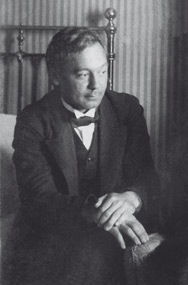
\includegraphics[scale=0.9]{images/Delone.jpg}
		\caption{Boris Nikolaevich Delone \\ πηγή: https://en.wikipedia.org/wiki/File:Delone\_cropped\_1924.jpg}
	\end{figure}
\end{frame}

\begin{frame}
	\frametitle{\en Delaunay \el Τριγωνοποίηση - Θεωρία}
	\begin{itemize}
		\item \el Παραδοχή: τα σημεία που πρόκειται να τριγωνοποιηθούν βρίσκονται σε γενική θέση.
		\item \el Γενική θέση: τέσσερα σημεία δε βρίσκονται πάνω στον ίδιο κύκλο.
		\item \el Ακολουθούν δύο προσεγγίσεις της θεωρίας για την τριγωνοποίηση \en Delaunay:
		\begin{itemize}
			\item \el Βάση γωνιών και ακμών
			\item \el Βάση κύκλων
		\end{itemize}
	\end{itemize}
\end{frame}

\begin{frame}
	\frametitle{\en Delaunay \el Τριγωνοποίηση - Θεωρία - Βάση γωνιών και ακμών}
	\begin{itemize}
		\item \el Διάνυσμα γωνιών (\(A(T)\)): διάνυσμα που περιέχει όλες τις γωνίες της τριγωνοποίησης.
		\item \el Αν το πλήθος των τριγώνων είναι \(m\), τότε το πλήθος των γωνιών είναι \(3m\).
		\item \el 
		\begin{align}
		A(T) := (a_1, a_2, ..., a_{3m})
		\end{align}
		όπου
		\begin{align}
		a_i \leq a_j \text{, } \forall i<j
		\end{align}
	\end{itemize}
\end{frame}

\begin{frame}
	\frametitle{\en Delaunay \el Τριγωνοποίηση - Θεωρία - Βάση γωνιών και ακμών}
	\begin{itemize}
		\item \el Αν \(Τ'\) είναι μια διαφορετική τριγωνοποίηση για το ίδιο σύνολο σημείων \(P\) και το αντίστοιχο διάνυσμα γωνιών είναι το \(A(T') = (a_{1}', a_{2}', ..., a_{3m}')\), θα λέμε ότι \(Α(Τ) > Α(Τ')\) αν υπάρχει \(i\), όπου \(1 \leq i \leq 3m\) τέτοιο ώστε 
		\begin{align*}
		a_j = a_{j}' \text{, } \forall j < i \text{ και } a_i > a_{i}'
		\end{align*}
		\item \el Στόχος είναι να καταφέρουμε να εντοπίσουμε το μεγαλύτερο διάνυσμα γωνιών.
		
	\end{itemize}
\end{frame}

\begin{frame}
	\frametitle{\en Delaunay \el Τριγωνοποίηση - Θεωρία - Βάση γωνιών και ακμών}
	\begin{mydefinition}{Παράνομη ακμή}{}
		Έστω \(T\) μία τριγωνοποίηση των σημείων \(P\).  Καλούμε μία ακμή "παράνομη" εαν μπορούμε να αυξήσουμε τη μικρότερη γωνία του διανύσματος γωνιών κάνοντάς την flip.
	\end{mydefinition}
	\begin{itemize}
		\item \el Αν \(T\) μία τριγωνοποίηση που περιέχει μία παράνομη ακμή και \(T'\) η τριγωνοποίηση που έχει γίνει \en flip \el η παράνομη ακμή, τότε: \(A(T') \geq A(T)\)
	\end{itemize}
	\begin{mydefinition}{Νόμιμη Τριγωνοποίηση}{}
		Μία τριγωνοποίηση \(T\) καλείται νόμιμη εαν δεν περιέχει καμία παράνομη ακμή.
	\end{mydefinition}
\end{frame}

\begin{frame}
	\frametitle{\en Delaunay \el Τριγωνοποίηση - Θεωρία - Βάση γωνιών και ακμών}
	\begin{mydefinition}{Τριγωνοποίηση Delaunay}{}
		Για ένα σύνολο σημείων \(P\) στο επίπεδο, η τριγωνοποίηση Delaunay είναι η τριγωνοποίηση εκείνη που δεν περιέχει καμία παράνομη ακμή. Συμβολίζουμε την τριγωνοποίηση Delaunay των σημείων με \(Del(P)\).
	\end{mydefinition}
\end{frame}

\begin{frame}
	\frametitle{\en Delaunay \el Τριγωνοποίηση - Θεωρία - Βάση κύκλων}
	\begin{mytheorem}{Γωνίες που βαίνουν σε χορδή}{}
		Έστω \(C\) να είναι ένας κύκλος και \(l\) μία ευθεία που τέμνει τον κύκλο στα σημεία \(a\) και \(b\). Έστω \(p\) και \(q\) σημεία πάνω στην περίμετρο του κύκλου. Τότε η γωνία που βαίνει στο τόξο \(ab\) με κορυφή το σημείο \(p\) είναι ίση με την γωνία που βαίνει στο ίδιο τόξο και έχει κορυφή το σημείο \(q\). 
	\end{mytheorem}
	\begin{columns}
		\column{0.5\textwidth}
		\begin{figure}
			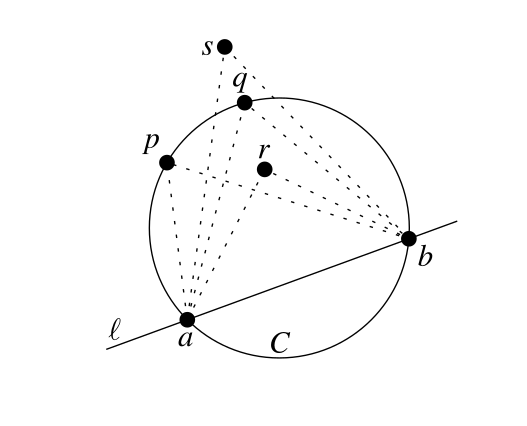
\includegraphics[scale=0.25]{images/circle.png}
		\end{figure}
		\column{0.5\textwidth}
		\begin{figure}
			\caption{Κύκλος C με τόξο ab \\ πηγή: "Computational Geometry, Algorithms and Applications,Third Edition", σελ. 194}
		\end{figure}
	\end{columns}
\end{frame}

\begin{frame}
	\frametitle{\en Delaunay \el Τριγωνοποίηση - Θεωρία - Βάση κύκλων}
	\begin{mytheorem}{Γωνίες που βαίνουν σε χορδή}{}
		Έστω \(C\) να είναι ένας κύκλος και \(l\) μία ευθεία που τέμνει τον κύκλο στα σημεία \(a\) και \(b\). Έστω \(r\) ένα σημείο εντός του κύκλου και \(s\) ένα σημείο εκτός. Τότε η γωνία που βαίνει στο τόξο \(ab\) με κορυφή το σημείο \(r\) είναι μεγαλύτερη από την γωνία που βαίνει στο ίδιο τόξο και έχει κορυφή το σημείο \(s\). 
	\end{mytheorem}
	\begin{columns}
		\column{0.5\textwidth}
		\begin{figure}
			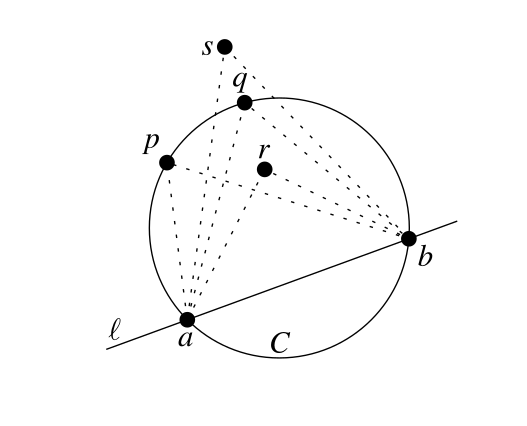
\includegraphics[scale=0.25]{images/circle.png}
		\end{figure}
		\column{0.5\textwidth}
		\begin{figure}
			\caption{Κύκλος C με τόξο ab \\ πηγή: "Computational Geometry, Algorithms and Applications,Third Edition", σελ. 194}
		\end{figure}
	\end{columns}
\end{frame}

\begin{frame}
	\frametitle{\en Delaunay \el Τριγωνοποίηση - Θεωρία - Βάση κύκλων}
	\begin{mylemma}{}{}
		Έστω \(C\) ένας κύκλος και \(p_i, p_j, p_k\) σημεία πάνω στον κύκλο και \(p_l\) σημείο εντός του κύκλου. Αν τα \(p_i, p_j, p_k, p_l\) σχηματίζουν ένα κυρτό πολύγωνο, τότε αυτό μπορεί να τριγωνοποιηθεί και να παραχθούν τα τρίγωνα \(p_i p_j p_k\) και \(p_i p_j p_l\) με κοινή ακμή την \(p_i p_j\). Η ακμή \(p_i p_j\) είναι παράνομη.
	\end{mylemma} 	
	\begin{mylemma}{}{}
		Έστω \(C\) ένας κύκλος και \(p_i, p_j, p_k\) σημεία πάνω στον κύκλο και \(p_l\) σημείο εκτός του κύκλου. Αν τα \(p_i, p_j, p_k, p_l\) σχηματίζουν ένα κυρτό πολύγωνο, τότε αυτό μπορεί να τριγωνοποιηθεί και να παραχθούν τα τρίγωνα \(p_i p_j p_k\) και \(p_i p_j p_l\) με κοινή ακμή την \(p_i p_j\). Η ακμή \(p_i p_j\) είναι νόμιμη.
	\end{mylemma} 
\end{frame}

\begin{frame}
	\frametitle{\en Delaunay \el Τριγωνοποίηση - Θεωρία - Βάση κύκλων}
	\begin{mytheorem}{Η ιδιότητα των κενών κυκλων}{}
		Έστω \(P\) ένα σύνολο σημείων στο επίπεδο που βρίσκονται σε γενική θέση. Μία τριγωνοποίηση \(T\) είναι τριγωνοποίηση Delaunay αν και μόνο αν ο κυκλος που σχηματίζεται από κάθε τριάδα σημείων που αποτελούν τρίγωνο της τριγωνοποίησης δεν περιέχει κανένα άλλο σημείο του \(P\) στο εσωτερικό του.
	\end{mytheorem} 
\end{frame}

\begin{frame}
	\frametitle{\en Delaunay \el Τριγωνοποίηση - Θεωρία - Βάση κύκλων}
	\begin{mytheorem}{Delaunay Τριγωνοποίηση}{}
		Σε μία τριγωνοποίηση Delaunay \(T\) των σημείων \(P\): \\
		1. Τρία σημεία κατασκευάζουν τρίγωνο αν και μόνο αν ο περιγεγραμμένος ανοιχτός κύκλος του δεν περιέχει κανένα άλλο σημείο του \(P\). \\
		2. Δύο σημεία κατασκευάζουν ακμή αν και μόνο αν υπάρχει κύκλος με τα σημεία αυτά στην περιφέρειά του που δεν περιέχει κανένα άλλο σημείο του \(P\) 	
	\end{mytheorem}
\end{frame}

\begin{frame}
	\frametitle{\en Delaunay \el Τριγωνοποίηση - Κατασκευή}
	\begin{itemize}
		\item \el Παρουσιάζουμε τον αυξητικό αλγόριθμο κατασκευής \en Delaunay \el Τριγωνοποίησης.
		\item \el Λαμβάνει ένα σύνολο σημείων και σε κάθε βήμα εξετάζει ενα απο τα σημεία αυτά και παράγει την τρέχουσα Delaunay τριγωνοποίηση, μέχρι που εξετάζει όλο το σύνολο σημείων.
		\item \el Η επιλογή σημείου σε κάθε βήμα γίνεται με τυχαίο τρόπο.
		\item \el Μέση πολυπλοκότητα: \(Ο(n logn)\) 
		\item \el Χείριστη περίπτωση: \(O(n^2)\).
	\end{itemize}
\end{frame}

\begin{frame}
	\frametitle{\en Delaunay \el Τριγωνοποίηση - Κατασκευή}
	\begin{itemize}
		\item \el Επιλέγει 3 σημεία στο επίπεδο των οποίων το αντίστοιχο τρίγωνο περιλαμβάνει όλα τα σημεία προς τριγωνοποίηση. 
		\item \el Για κάθε σημείο που ελέγχει εντόπίζει αν βρίσκεται
		\begin{itemize}
			\item \el εντός τριγώνου της ήδη κατασκευασμένης τριγωνοποίησης
			\begin{itemize}
				\item \el Κατασκευάζονται τρείς νέες ακμές, οι οποίες εκτείνονται από το υπό εξέταση σημείο προς την κάθε κορυφή του τριγώνου που το περιέχει. 
			\end{itemize}
			\item \el πάνω σε κάποια ακμής της τριγωνοποίησης.
			\begin{itemize}
				\item \el Η ακμή αυτή είναι κοινή ακμή για δύο τριγωνα. 
				\item \el Δημιουργούνται δύο νέες ακμές από το σημείο που εξετάζεται προς τη μία κορυφη του ενός και του άλλου τριγώνου που δεν ανήκουν στο ευθύγραμμο τμήμα.
			\end{itemize}
		\end{itemize}  
	 	\item \el Ελέγχει ότι η τριγωνοποίηση είναι 
	 	\en Delaunay, \el διότι η προσθήκη μιας νέας ακμής μπορεί να κάνει παράνομες τις ήδη υπάρχουσες ακμές της τριγωνοποίησης και κάνει κατάλληλα flips.
	\end{itemize}
\end{frame}

\begin{frame}
	\frametitle{\en Delaunay \el Τριγωνοποίηση - Κατασκευή}
	\begin{figure}
		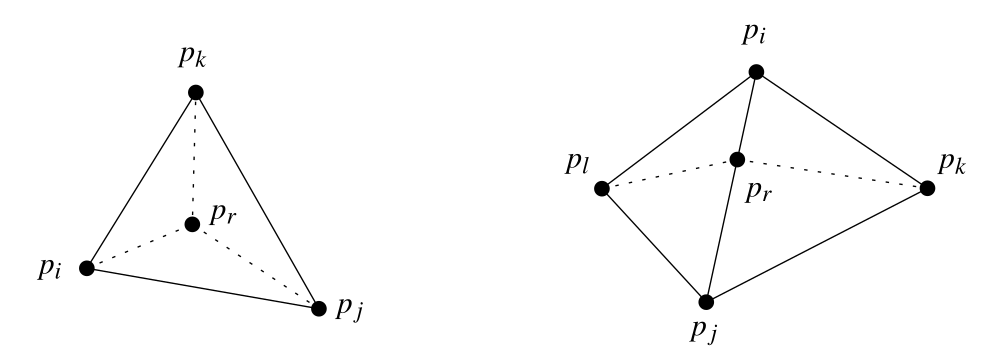
\includegraphics[scale=0.3]{images/incremental.png}
		\caption{Οι δύο περιπτώσεις που εξετάζει ο αυξητικός αλγόριθμος κατά την εισαγωγή ενός νέου σημείου \(p_r\). Αριστερά φαίνεται η πρώτη περίπτωση, όπου το νεό σημείο εντοπίζεται εντός τριγώνου της τριγωνοποίησης, ενώ δεξία φαίνεται η δεύτερη περίπτωση όπου το νέο σημείο βρίσκεται πάνω σε ακμή της τριγωνοποίησης \\ πηγή: "Computational Geometry, Algorithms and Applications, Third Edition", σελ.: 200}
	\end{figure}
\end{frame}

\subsubsection{Κυρτό περίβλημα}
\begin{frame}
	\frametitle{\el Θεωρητική Προσέγγιση}
	\tableofcontents[currentsubsection]
\end{frame}
\begin{frame}
	\frametitle{\el Κυρτό Περίβλημα}
	\begin{itemize}
		\item \el Πολλές φορές είναι απαραίτητο, δοθέντος ενός συνόλου σημείων να βρεθεί ένα κυρτό περίβλημα που να περιέχει όλα τα σημεία στο εσωτερικό του.
		\item \el Εμείς θα επικεντρωθούμε στην περίπτωση όπου τα σημεία ανήκουν στο επίπεδο.
	\end{itemize}	
	\begin{mydefinition}{Κυρτό}{}
		Κυρτό (convex) είναι κάθε αντικείμενο ή σύνολο σημείων, στο οποίο κάθε ευθύγραμμο τμήμα με άκρα που ανήκουν στο αντικείμενο ή στο σύνολο σημείων βρίσκεται μέσα στο αντικείμενο.
	\end{mydefinition}
	\begin{itemize}
		\item \el Στόχος είναι να βρεθεί μία κυρτή πολυγωνική γραμμή που να περιέχει όλα τα σημεία που επιθυμούμε.
	\end{itemize}	
\end{frame}

\begin{frame}
	\frametitle{\el Κυρτό Περίβλημα}
	\begin{itemize}
		\item \el Η πολυγωνική γραμμή πρέπει να είναι κλειστή.
	\end{itemize}	
	\begin{mydefinition}{Κλειστή Πολυγωνική Γραμμή}{}
		Κλειστή πολυγωνική γραμμή καλείται η πολυγωνική γραμμή της οποίας το τέλος του τελευταίου τμήματος ταυτίζεται με την αρχή του πρώτου.
	\end{mydefinition}
	\begin{mydefinition}{Κλειστό Πολύγωνο}{}
		Κλειστό πολύγωνο καλείται η ένωση μιας κλειστής πολυγωνικής γραμμής και του εσωτερικού της.
	\end{mydefinition}		
\end{frame}

\begin{frame}
	\frametitle{\el Κυρτό Περίβλημα}
	\begin{mydefinition}{Κυρτό Περίβλημα}{}
		Το κυρτό περίβλημα ενός συνόλου σημείων στο επίπεδο είναι το κυρτό πολύγωνο με ελάχιστο εμβαδόν που περιλαμβάνει όλα τα δεδομένα σημεία.
	\end{mydefinition}	
	\begin{mydefinition}{Κυρτό Περίβλημα}{}
		Το κυρτό περίβλημα (convex hull) ενός συνόλου σημείων στο επίπεδο είναι το κυρτό πολύγωνο που περιέχει τα δεδομένα σημεία και είναι ελάχιστο ως προς τη σχέση υποσυνόλου σημείων. Δεν υπάρχει κυρτό πολύγωνο που να περιέχει όλα τα δεδομένα σημεία και να είναι γνήσιο υποσύνολο του κυρτού περιβλήματος.
	\end{mydefinition}	
\end{frame}

\begin{frame}
	\frametitle{\el Κυρτό Περίβλημα}
	\begin{figure}
		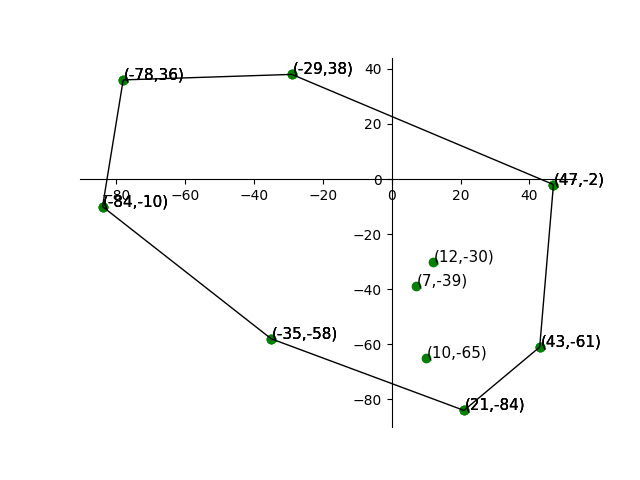
\includegraphics[scale=0.5]{images/convexhull.png}
		\caption{Παράδειγμα convex hull δέκα σημείων στο επίπεδο \\ πηγή: Output αλγορίθμου που έχουμε υλοποιήσε για την εύρεση κυρτού περιβλήματος}
	\end{figure}
\end{frame}

\begin{frame}
	\frametitle{\el Κυρτό Περίβλημα - Κατασκευή}
	\begin{itemize}
		\item \el Αυξητικός αλγόριθμος
		\item \el Αλγόριθμος περιτύλιξης
	\end{itemize}
\end{frame}

\subsection{Γραφοθεωρητική Προσέγγιση}
\begin{frame}
	\frametitle{\el Θεωρητική Προσέγγιση}
	\tableofcontents[currentsubsection]
\end{frame}

\begin{frame}
	\frametitle{\el Γραφοθεωρητική Προσέγγιση}
	\begin{itemize}
		\item \el Το \en TSP \el είναι μία επέκταση του προβλήματος εύρεσης κυκλώματος \en Hamilton.
		\item \el Το \en TSP \el αναζητά ένα κύκλωμα \en Hamilton \el με ελάχιστο μήκος.
		\item \el Θεωρούμε το γράφημα του χαρτη των πόλεων και των αντίστοιχων διαδρομών να είναι το \(G = (V,E,w(i,j))\)
		\item \el \(V\): πόλεις (κορυφές)
		\item \el \(E\) : διαδρομές μεταξύ δύο πόλεων (ακμές) 
		\item \el \(w\): μήκος διαδρομής από την πόλη \(i\) στην πόλη \(j\) (το βάρος της ακμής \((i,j)\))
		
		\begin{align}
		w:E \rightarrow \R^{+}
		\end{align} 	
		τέτοια ώστε να ισχύει 
		\begin{align}
		w(i,k) \leq w(i,j) + w(j,k)
		\end{align} 
	\end{itemize}
\end{frame}

\begin{frame}
	\frametitle{\el Γραφοθεωρητική Προσέγγιση}
	\begin{center}
		\scalebox{0.9}{
			\begin{minipage}{0.9\linewidth}
				\begin{algorithm}[H]
				\SetAlgoLined
				\KwResult{Κύκλωμα Hamilton για το πρόβλημα του περιοδέυοντος πωλητή}
				
				Επέλεξε αυθαίρετα μία κορυφή v \;
				Ανέθεσε την v στην x \;
				\For{x} 
				{Επέλεξε μία κορυφή v που δεν βρίσκεται στο μονοπάτι και απέχει τη μικρότερη απόσταση από την τρέχουσα x \;
					Πρόσθεσε την ακμή (x,v) στο μονοπάτι \;
					Ανανέωσε την x με την v \;}
				Σχημάτισε κύκλωμα συνδέοντας την αρχική κορυφή με την τελική κορυφή του μονοπατιού \;
				
				\caption{Μέθοδος πλησιέστερου γείτονα}
			\end{algorithm}
			\end{minipage}
		}
	\end{center}
\end{frame}

\subsection{Γεωμετρική Προσέγγιση}
\begin{frame}
	\frametitle{\el Θεωρητική Προσέγγιση}
	\tableofcontents[currentsubsection]
\end{frame}

\begin{frame}
	\frametitle{\el Γεωμετρική Προσέγγιση}
	\begin{itemize}
		\item \el Γεωμετρικοί αλγόριθμοι εύρεσης μονοπατιού για το \en TSP:
		\begin{itemize}
			\item \el Αλγόριθμος Σύγκρισης Γωνιών
			\item \el Αλγόριθμος Σύγκρισης Ελλείψεων
			\item \el Αλγόριθμος με τριγωνοποίηση \en Delaunay
		\end{itemize}
	\end{itemize}
\end{frame}

\begin{frame}
	\frametitle{\el Γεωμετρική Προσέγγιση - Αλγόριθμος Σύγκρισης Γωνιών}
	\begin{itemize}
		\item \el Η βασική ιδέα του αλγορίθμου είναι, δοθέντος ενός συνόλου σημείων στον Ευκλείδιο χώρο, να σχεδιάστεί μονοπάτι που προσεγγίζει το βέλτιστο μονοπάτι για τον πλανόδιο πωλητή.
		\item \el  Δεν παράγει οπωσδήποτε το βέλτιστο μονοπάτι.
	\end{itemize}
	\begin{figure}
		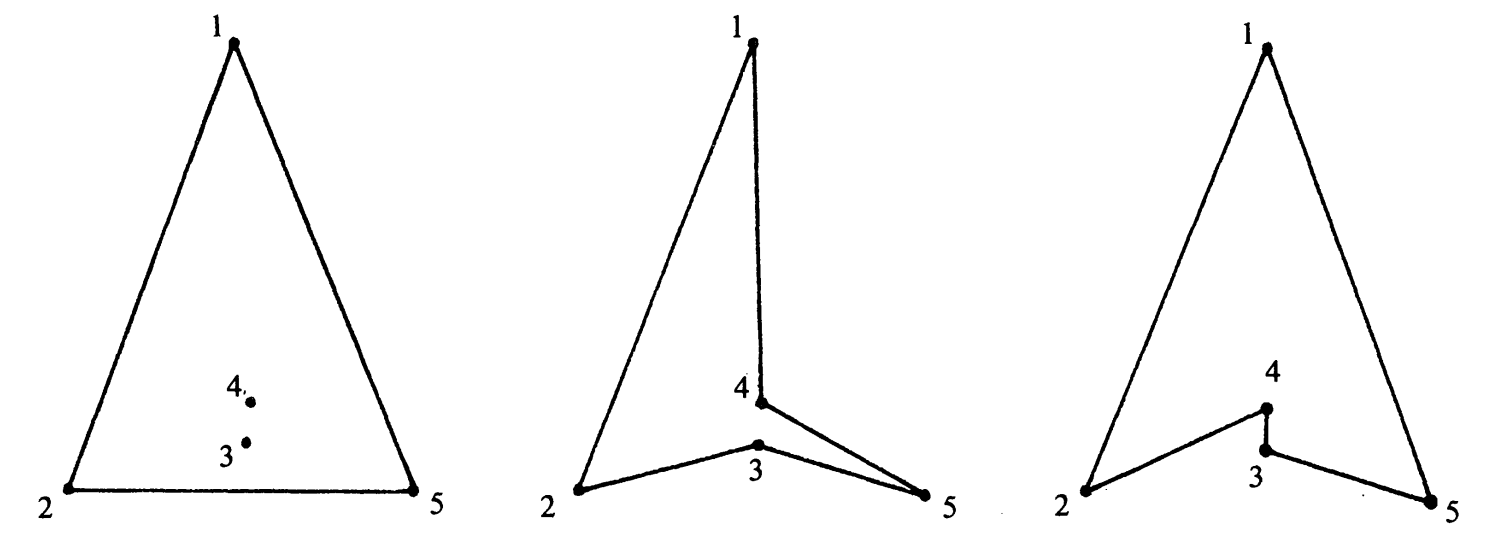
\includegraphics[scale=0.2]{images/geometric_approach_angle5.png}
		\caption{Παράδειγμα παραγωγής μη βέλτιστου μονοπατιού. Ο αλγόριθμος δίνει το αποτέλεσμα που φαίνεται στη μέση, ενώ το βέλτιστο αποτέλεσμα φαίνεται στα δεξία.\\ πηγή: \cite{16}}
	\end{figure}
\end{frame}

\begin{frame}
	\frametitle{\el Γεωμετρική Προσέγγιση - Αλγόριθμος Σύγκρισης Γωνιών}
	\begin{itemize}		
		\item \el  Πρώτο βήμα: εύρεση του κυρτού περιβλήματος των σημείων 
		\item \el Το κυρτό περίβλημα είναι μία πρώτη μορφή του τελικού μονοπατιού \en ("partial μονοπάτι").
	\end{itemize}
	\begin{figure}
		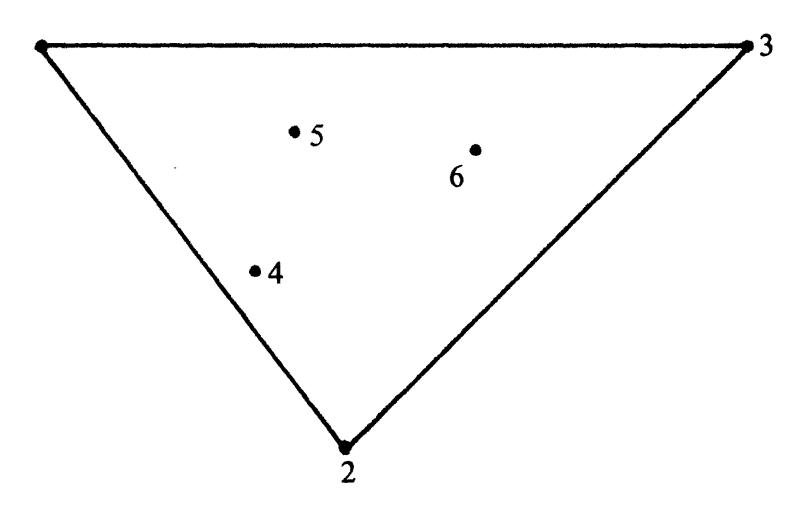
\includegraphics[scale=0.2]{images/geometric_approach_angle1.png}
		\caption{Οι "εσωτερικές" πόλεις είναι τα σημεία με label 4,5 και 6. Οι "εξωτερικές" πόλεις βρίσκονται στο convex hull (partial μονοπάτι)\\ πηγή: \cite{16}}
	\end{figure} 
\end{frame}

\begin{frame}
	\frametitle{\el Γεωμετρική Προσέγγιση - Αλγόριθμος Σύγκρισης Γωνιών}
	\begin{itemize}		
		\item \el Δεύτερο βήμα: ενσωμάτωση των εσωτερικών πόλεων στο μονοπάτι.
		\item \el Διαδοχικές επαναλήψεις μέχρι να έχουν ενσωματωθεί στο μονοπάτι όλες οι εσωτερικές πόλεις.
		\item \el Σε κάθε επανάληψη ενσωματώνεται και μία νέα εσωτερική πόλη στο μονοπάτι. 
	\end{itemize}
\end{frame}

\begin{frame}
	\frametitle{\el Γεωμετρική Προσέγγιση - Αλγόριθμος Σύγκρισης Γωνιών}
	\begin{itemize}		
		\item \el Σχηματίζουμε όλες τις γωνίες των οποίων η κορυφή είναι ένα από τα εσωτερικά σημεία και οι δύο αντίστοιχες πλευρές βαίνουν από δύο διαδοχικά σημεία του \en convex hull.
		\item \el Επιλέγεται η γωνία που έχει το μεγαλύτερο μέτρο.
		\item \el Η αντίστοιχη κορυφή - πόλη ενσωματώνεται στο μονοπάτι μαζί με τις δύο πλευρές της γωνίας
		\item \el Η διαδικασία επαναλαμβάνεται μέχρι όλες οι εσωτερικές πόλεις να έχουν ενσωματωθεί στο μονοπάτι.
	\end{itemize}
\end{frame}

\begin{frame}
	\frametitle{\el Γεωμετρική Προσέγγιση - Αλγόριθμος Σύγκρισης Γωνιών}
	\begin{columns}
		\begin{column}{0.3\textwidth}
			\begin{figure}
				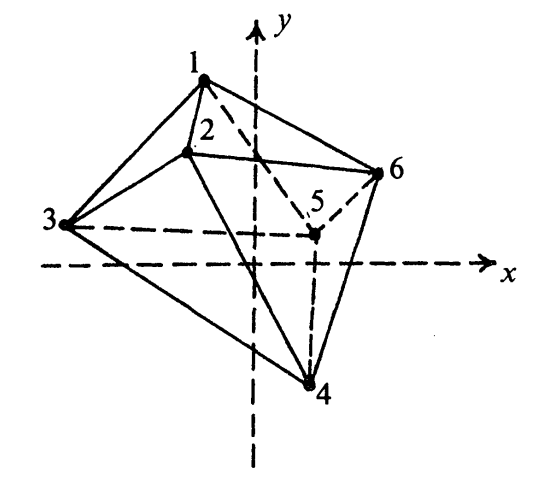
\includegraphics[scale=0.2]{images/geometric_approach_angle2.png}
				\caption{Έχει κατασκευαστεί το convex hull και οι τέσσερεις γωνίες για κάθε μία από τις δύο εσωτερικές πόλεις. \\ πηγή: \cite{16}}
			\end{figure} 
		\end{column}
		\begin{column}{0.3\textwidth}
			\begin{figure}
				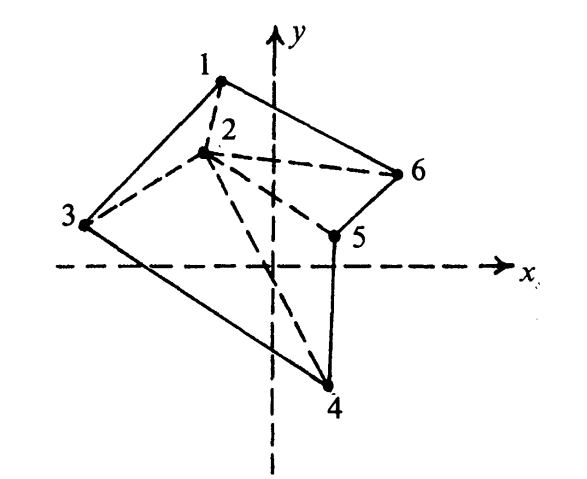
\includegraphics[scale=0.2]{images/geometric_approach_angle3.png}
				\caption{Η μεγαλύτερη γωνία ανήκει στο σημείο 5. Το σημείο 5 ενσωματώνεται στο partial μονοπάτι. \\ πηγή: \cite{16}}
			\end{figure} 
		\end{column}
		\begin{column}{0.3\textwidth}
			\begin{figure}
				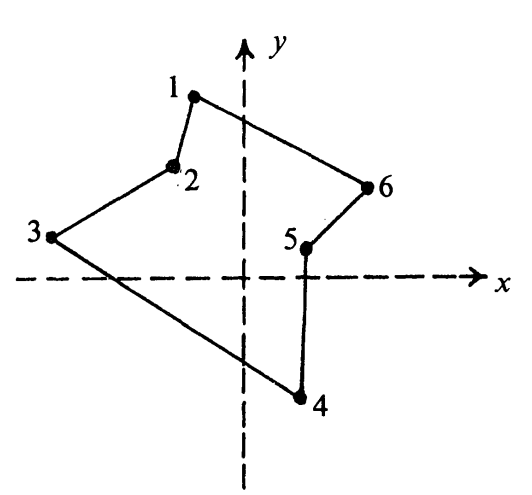
\includegraphics[scale=0.2]{images/geometric_approach_angle4.png}
				\caption{Το σημείο 2 είναι το τελευταίο και ενσωματώνεται στο μονοπάτι, δίοτι περιέχει τη μεγαλύτερη γωνία\\ πηγή: \cite{16}}
			\end{figure} 
		\end{column}	
	\end{columns}
\end{frame}

\begin{frame}
	\frametitle{\el Γεωμετρική Προσέγγιση - Αλγόριθμος Σύγκρισης Γωνιών}
	\begin{itemize}		
		\item \el Το μέτρο της γωνίας \(α\) που σχηματίζεται μεταξύ δύο διανυσμάτων \(u\) και \(v\) μπορεί να βρεθεί από τη σχέση
		\begin{align*}
		u \cdot v = |u||v|\cos α
		\end{align*}
	\end{itemize}
\end{frame}

\begin{frame}
	\frametitle{\el Γεωμετρική Προσέγγιση - Αλγόριθμος Σύγκρισης Γωνιών}	
	\begin{center}
		\scalebox{0.9}{
			\begin{minipage}{0.9\linewidth}
				\begin{algorithm}[H]
					\SetAlgoLined
					\KwIn{Σύνολο σημείων s στον Ευκλείδιο χώρο}
					\KwResult{Μονοπάτι για το TSP}
					
					partial\_tour = convex hull των s \;
					out\_points = Σημεία που βρίσκονται στο convex hull \; 
					in\_points = s - out\_points \;
					
					\While{in\_points \(\neq \emptyset\)}
					{
						\For{i} 
						{
							Κατασκεύασε όλες τις γωνίες με κορυφή το σημείο in\_points[i] και πλευρές που τέμνουν δύο διαδοχικά σημεία του partial\_tour \; 
							Υπολόγισε το μέτρο των γωνιών και αποθήκευσε τη μεγαλύτερη γωνία \;
						}
						partial\_tour += εσωτερικό σημείο με μεγαλύτερη γωνία \;
					}
					
					\caption{Εύρεση μονοπατιού TSP με το μέτρο γωνιών}
				\end{algorithm}
			\end{minipage}
		}
	\end{center}
\end{frame}

\begin{frame}
	\frametitle{\el Γεωμετρική Προσέγγιση - Αλγόριθμος Σύγκρισης Ελλείψεων}
	\begin{itemize}
		\item \el Εύρεση του \en convex hull (partial μονοπάτι).
		\item \el  Σε κάθε επανάληψη ενσωματώνεται μόνο μία καινούρια εσωτερική πόλη στο μονοπάτι
		\item \el Ο αλγόριθμος τερματίζει όταν όλες οι εσωτερικές πόλεις περιέχονται στο μονοπάτι του πλανόδιου πωλητή. \\
		\item \el Η επιλογή της πόλης που θα ενσωματωθεί στο \en partial \el μονοπάτι γίνεται με τη βοήθεια ελλείψεων.
	\end{itemize}
\end{frame}

\begin{frame}
	\frametitle{\el Γεωμετρική Προσέγγιση - Αλγόριθμος Σύγκρισης Ελλείψεων}
	\begin{itemize}
		\item \el Σε κάθε επανάληψη δημιουργούνται όλες οι ελλείψεις που έχουν εστίες δύο διαδοχικά σημεία του \en convex hull \el και βαίνουν από ένα εσωτερικό σημείο.
		\item \el Για κάθε μία από τις ελλείψεις υπολογίζεται η εκκεντρότητά της.
		\item \el  Επιλέγεται το σημείο που ανήκει στην έλλειψη με τη μεγαλύτερη εκκεντρότητα (λιγότερο κυκλική μορφή).
	\end{itemize}
	\begin{figure}
		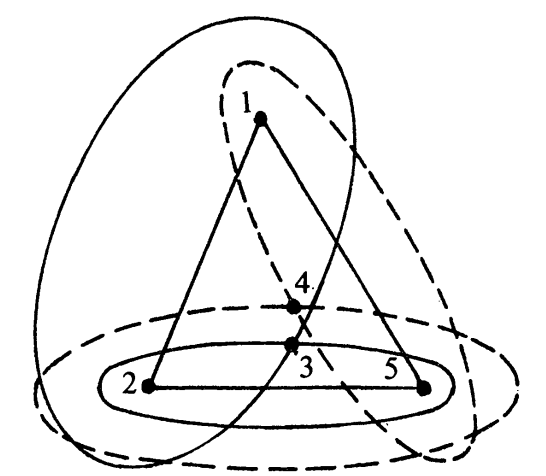
\includegraphics[scale=0.15]{images/geometric_approach_ellipse2.png}
		\caption{Στη φάση αυτή επιλέγεται το εσωτερικό σημείο με label 3, διότι ανήκει στην έλλειψη με τη μεγαλύτερη εκκεντρότητα.\\ πηγή: \cite{16}}
	\end{figure}  
\end{frame}

\begin{frame}
	\frametitle{\el Γεωμετρική Προσέγγιση - Αλγόριθμος Σύγκρισης Ελλείψεων}
	\begin{itemize}
		\item \el Εκκεντρότητα:
		\begin{align*}
		e = \frac{d_3}{d_1 + d_2}
		\end{align*}
		όπου \(d_3\) είναι η απόσταση μεταξύ των δύο εστιών και \(d_1, d_2\) είναι η απόσταση μεταξύ ενός σημείου της έλλειψης και των δύο εστιών αντίστοιχα.
	\end{itemize}
	\begin{figure}
		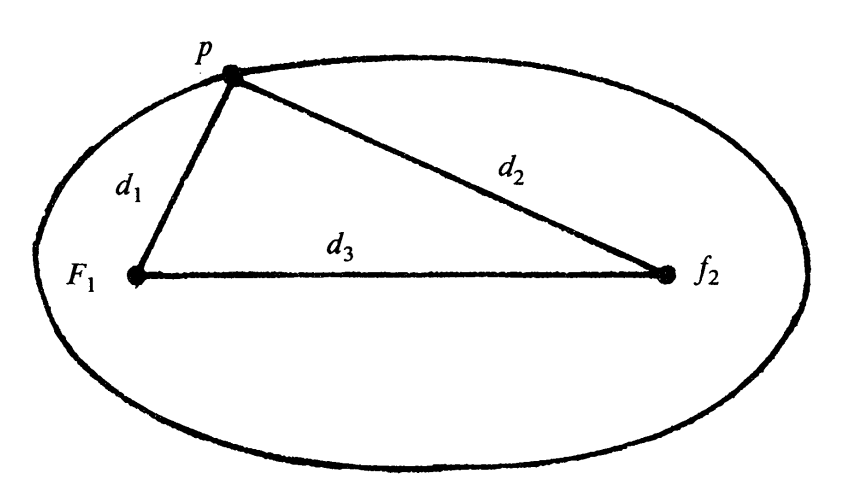
\includegraphics[scale=0.2]{images/geometric_approach_ellipse1.png}
		\caption{Η εκκεντρότητα δίνεται από τον τύπο \(e = \frac{d_3}{d_1 + d_2}\)\\ πηγή: \cite{16}}
	\end{figure}
\end{frame}

\begin{frame}
	\frametitle{\el Γεωμετρική Προσέγγιση - Αλγόριθμος Σύγκρισης Ελλείψεων}	
	\begin{center}
		\scalebox{0.9}{
			\begin{minipage}{0.9\linewidth}
				\begin{algorithm}[H]
					\SetAlgoLined
					\KwIn{Σύνολο σημείων s στον Ευκλείδιο χώρο}
					\KwResult{Μονοπάτι για το TSP}
					
					partial\_tour = convex hull των s \;
					out\_points = Σημεία που βρίσκονται στο convex hull \;
					in\_points = s - out\_points \;
					
					\While{in\_points \(\neq \emptyset\)}
					{
						\For{i} 
						{
							Κατασκεύασε όλες τις ελλείψεις με εστίες δύο διαδοχικά σημεία του partial\_tour που βαίνουν από το  in\_points[i] \; 
							Υπολόγισε την εκκεντρότητα όλων των ελλείψεων και αποθήκευσε τη μεγαλύτερη \;
						}
						partial\_tour += σημείο που ανήκει στην έλλειψη με τη μεγαλύτερη εκκεντρότητα \;
					}
					
					\caption{Εύρεση μονοπατιού TSP με την εκκεντρότητα ελλείψεων}
				\end{algorithm}
			\end{minipage}
		}
	\end{center}
\end{frame}

\begin{frame}
	\frametitle{\el Γεωμετρική Προσέγγιση - Αλγόριθμος με τριγωνοποίηση \en Delaunay}
	\begin{itemize}
		\item \el 
	\end{itemize}
\end{frame}

\begin{frame}
	\frametitle{\el Γεωμετρική Προσέγγιση - Αλγόριθμος με τριγωνοποίηση \en Delaunay}
	\begin{itemize}
		\item \el 
	\end{itemize}
\end{frame}

\begin{frame}
	\frametitle{\el Γεωμετρική Προσέγγιση - Αλγόριθμος με τριγωνοποίηση \en Delaunay}
	\begin{itemize}
		\item \el 
	\end{itemize}
\end{frame}

\subsection{Ειδικές Περιπτώσεις \en TSP}
\begin{frame}
	\frametitle{\el Θεωρητική Προσέγγιση}
	\tableofcontents[currentsubsection]
\end{frame}

\begin{frame}
	\frametitle{\el Ειδικές Περιπτώσεις \en TSP}
	
\end{frame}

\section{Υλοποίηση}
\subsection{title}
\begin{frame}
	\frametitle{\el Υλοποίηση}
	\tableofcontents[currentsubsection]
\end{frame}
\begin{frame}
	\frametitle{\en title}
	
\end{frame}

\section{Βιβλιογραφία}
\begin{frame}
	\frametitle{Βιβλιογραφία}
	\begin{itemize}
		\item \textit{\en Exact and Approximation Algorithms for Time-Window TSP, 
			Jie Gao, Su Jia, Joseph S. B. Mitchell,
			CG:YRF, Boston, MA, USA, June 14-18, 2016}
		\item \textit{\en An O ( n log n ) Heuristic for the Euclidean Traveling Salesman Problem, 
			Evgeny Yanenko, Eckart
		Schuhmacher, Ulrich Spörlein, Kurt Tutschku,	April 25, 2005}
		\item \textit{Approximation Algorithms for Time-Window TSP and Prize Collecting TSP Problems,
			Jie Gao, Su Jia, Joseph S. B. Mitchell, Lu Zhao,
			Stony Brook University, Stony Brook, NY 11794, USA.}
		\item \text{\en Applications of the TSP,} \\
		\text{http://www.math.uwaterloo.ca/tsp/apps/index.html}	
\end{itemize}
\end{frame}

\begin{frame}
	\frametitle{Βιβλιογραφία}
	\begin{itemize}
		\item \textit{\el Εισαγωγή στους αλγορίθμους, Δεύτερη έκδοση, \en Thomas H. Cormen, Charles E. Leiserson, Ronald L. Rivest, Clifford Stein, \el Πανεπιστημιακές εκδόσεις Κρήτης, 2011, \en ISBN: 978-960-524-473-6}
		\item \textit{\el Τεχνητή Νοημοσύνη, Μία σύγχρονη προσέγγιση, Δεύτερη Αμερικανική έκδοση, \en Stuart Russel, Peter Norvig, \el σελ.: 101,	Κλειδάριθμος 2005, \en ISBN: 960-209-873-2}
		\item \textit{\el Στοιχεία διακριτών μαθηματικών, \en C. L. Liu, \el σελ.: 171-172, 178-179, 190-201, Πανεπιστημιακές εκδόσεις Κρήτης 2014, \en ISBN: 978-960-524-072-1}	
		\item \textit{\el Μαθηματικά Πληροφορικής, Ηλίας Κουτσουπιάς, σελ.: 112, Πανεπιστήμιο Αθηνών, Αθήνα, Οκτώβριος 2009}
	\end{itemize}
\end{frame}

\begin{frame}
	\frametitle{Βιβλιογραφία}
	\begin{itemize}
		\item \textit{\en Discrete and Computational Geometry, Satyan L. Devadoss, Joseph O'Rourke,
			\el σελ.: 81-86, \en Princeton University Press, 2011, ISBN: 978-0-691-14553-2}
		\item \textit{\en Computational Geometry,	Algorithms and Applications, Third Edition, 
			Mark de Berg, Otfried Cheong, Marc van Kreveld, Mark Overmars, \el σελ.: 193-204,
			\en Springer, 2008, ISBN: 978-3-540-77973-5}
		\item \textit{\el Υπολογιστική Γεωμετρία: Μια σύγχρονη αλγοριθμική προσέγγιση, Γιάννης Ζ. Εμίρης,
			σελ.: 199-208, Κλειδάριθμος, 2008, \en ISBN: 978-960-461-141-6 }
		\item \textit{\el Σχεδίαση και Ανάλυση Αλγορίθμων, Κωνσταντίνος Τσίχλας, Ιωάννης Μανωλόπουλος, Αναστάσιος Γούναρης, σελ.: 317-320, \en http://repfiles.kallipos.gr/html\_books/4410/contents.html ,2015
			ISBN: 978-960-603-465-7}	
	\end{itemize}
\end{frame}

\begin{frame}
	\frametitle{Βιβλιογραφία}
	\begin{itemize}
		\item \textit{\en Good triangulations yield good tours, Adam N. Letchford, Nicholas A. Pearson,
			Department of Management Science, Lancaster University, Lancaster LA1 4YW, UK, 4 May 2006}
		\item \textit{\en Geometric Approaches to solving the traveling salesman problem, John P. Norback, Robert 		F.Love, Managment Science, Vol. 23, No. 11, \el σελ.: 1208-1223, Ιούλιος 1977}
		\item \textit{\en The Convex-Hull-and-Line Traveling Salesman Problem: A Solvable Case,
			Vladimir G. Deineko, Rene van Dal, Gunter Rote,	Information Processing Letters 51 (1994), 
			\el σελ.: 141-148, Σεπτέμβριος 1992}
		\item \textit{\en Traveling Salesman Cycles are not always subgraphs of Delaunay triangulations or of Minimum 	weight triangulations,	Michael B. DILLENCOURT,	Computer Technology Associates, Inc., 7927 Jones Branch Drive, McLean, VA 22102, U.S.A, Communicated by Alan Shaw,	Received 23 October 1985, Revised 28 February 1986}
	\end{itemize}
\end{frame}

\end{document}